\hypertarget{cv:GestionarGlosario}{\section{Gestionar Mensajes}} \label{sec:GestionarMensajes}

	Esta funcionalidad le permitirá las acciones necesarias para controlar los mensajes y visualizarlos en una tabla en el proyecto sobre el que se está operando y solicitar el registro de uno nuevo.

		\subsection{Procedimiento}

			%Pasos de procedimiento
			\begin{enumerate}
				
			\item Ingrese a un proyecto existente desde la pantalla \ref{fig:GestionarProyectosColaborador}.
	
			\item Seleccione la opción \textbf{Mensajes} del menú \ref{fig:MN-LPC}.
	
			\item Se mostrará la pantalla \ref{fig:GestionarMensajes} ''Gestionar Mensajes''.

			%Pantalla
			\begin{figure}[h!]
				\begin{center}
					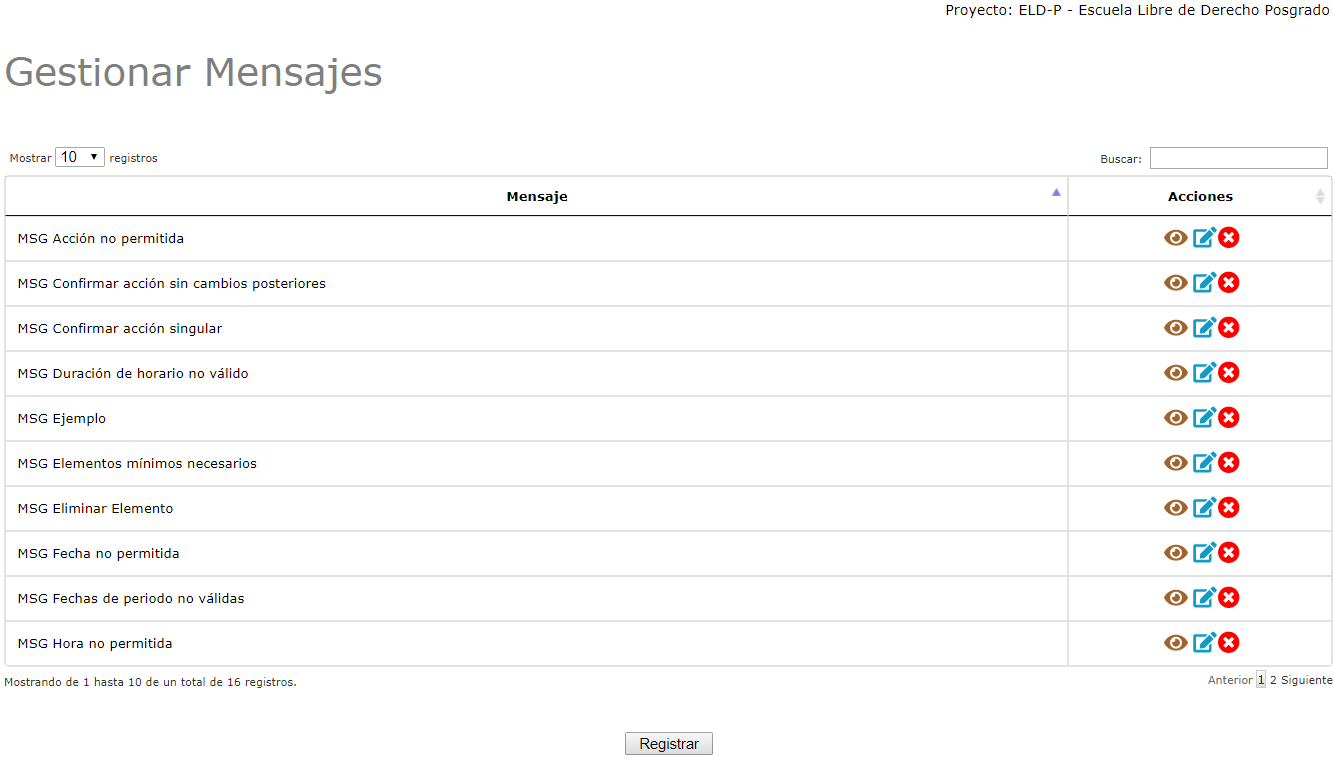
\includegraphics[scale=0.5]{roles/lider/mensajes/pantallas/IU9gestionarMensajes}
					\caption{Gestionar Mensajes}
					\label{fig:GestionarMensajes}
				\end{center}
			\end{figure}
		
				\item Seleccione la operación que desea realizar:
			
			Para (\hyperlink{cv:registrarMensaje}{Registrar}) dé clic en el botón \IURegistrar.
			
			Para (\hyperlink{cv:modificarTermino}{Modificar}) dé clic en el icono \IUEditar{} de algún término ya registrado.
			
			Para (\hyperlink{cv:eliminarProyecto}{Eliminar}) dé clic en el icono \IUBotonEliminar{} de algún término ya registrado.
			
			Para (\hyperlink{cv:consultarTermino}{Consultar}) dé clic en el icono \IUConsultar{} de algún término ya registrado.
			\end{enumerate}